%
% File acl2021.tex
%
%% Based on the style files for EMNLP 2020, which were
%% Based on the style files for ACL 2020, which were
%% Based on the style files for ACL 2018, NAACL 2018/19, which were
%% Based on the style files for ACL-2015, with some improvements
%%  taken from the NAACL-2016 style
%% Based on the style files for ACL-2014, which were, in turn,
%% based on ACL-2013, ACL-2012, ACL-2011, ACL-2010, ACL-IJCNLP-2009,
%% EACL-2009, IJCNLP-2008...
%% Based on the style files for EACL 2006 by 
%%e.agirre@ehu.es or Sergi.Balari@uab.es
%% and that of ACL 08 by Joakim Nivre and Noah Smith

\documentclass[11pt,a4paper]{article}
\usepackage[hyperref]{acl2021}
\usepackage{times}
\usepackage{latexsym}
\renewcommand{\UrlFont}{\ttfamily\small}

% This is not strictly necessary, and may be commented out,
% but it will improve the layout of the manuscript,
% and will typically save some space.
\usepackage{microtype}

\usepackage{multirow}
\usepackage{colortbl}
\usepackage{graphicx} %插入图片的宏包
\usepackage{float} %设置图片浮动位置的宏包
\usepackage{subfigure} %插入多图时用子图显示的宏包

%\aclfinalcopy % Uncomment this line for the final submission
%\def\aclpaperid{***} %  Enter the acl Paper ID here

%\setlength\titlebox{5cm}
% You can expand the titlebox if you need extra space
% to show all the authors. Please do not make the titlebox
% smaller than 5cm (the original size); we will check this
% in the camera-ready version and ask you to change it back.

\newcommand\BibTeX{B\textsc{ib}\TeX}

\title{Works based on NNLM}

\author{
    \textbf{Pingwei Sun} \\
    \\
    NEU-NLP Lab \\
    }

\date{}

\begin{document}
\maketitle
\begin{abstract}
During the second stage of our course, I have done work based on Neural Network Language Model.
Both a FFN and a RNN are built up.
As for further research, I have done some related works based on those models, which includes 
experiments on hyperparameters, comparing the performance of various models, introducing grad-clip and pre-train method.
The details of the works are presented as follows.

\end{abstract}


\section{Introduction}
With the improvement of computer processing ability, people have been exploring the method of processing natural language by programs.
One of the most important tasks is to create a language model, which can effectively generate a mathematical model according to our natural language.

The natural language model has gone through stages of the grammatical model, the statistical model and now stepped into the neural network stage.

Different from the previous dictionary-based theory, \textbf{NNLM}\citep{bengio2000neural} will transform natural language into a set of machine knowledge systems by learning from data. 
There are no artificial assumptions during the whole process and will also save a lot of storage costs.

However, it did not consider the sequential information of language.
To make models able to form memory, \textbf{RNN}\citep{mikolov2010recurrent} was launched representing history by neurons
with recurrent connections.

\textbf{Based on NNLM, I have conducted the following experiments:}
\begin{itemize}
\item Explore the impact of hyperparameters(step, embedded size, hidden size) on the performance of the model.
\item Compare performances of different models.
\item Introduce pretrained embedding parameters into the model.
\end{itemize}


\section{Methods}

\subsection{Vocabulary Construction}
Here I customize the method of constructing the vocabulary by myself. 
First, a document is opened by the program. Then the words are separated by space(ways of splitting can be changed by calling various APIs) and stored in a \emph{frequency dict} in the pattern of \emph{\{word:frequency\}}.

Then we need to build two \emph{dicts}, \emph{word2vecotr and vector2word}, to generate a dual-direct index. Special words such as \emph{[pad], [unk], [sos], [eos]} come first, and dual-direct index pairs are built according to the \emph{frequency dict}.

\subsection{Dataset Construction}
To feed the model with appropriate data, I rewrite the \emph{Dataset} method.
Specifically, the input corpus is translated into numbers according to the previous dual index sentence by sentence.
Then, \emph{[[n-input], [target]} corpus list are generated from sentences, following the instruction of \emph{n-step}, and those being unqualified in length will be padded in front. 
With the customized collate-fn, all records in the corpus list are packaged as tuples, gained by \emph{Dataloader} and finally make up batches. 

\subsection{Pretrain word embedding}
Pretraining word embedding \citep{mikolov2013efficient} is used in my program. With the help of \emph{gensim}, I gained a word-to-vector list based on the whole \emph{PTB} data set, which can be used to initialize the embedding layers in models. A test has also been done to see how it works.

\subsection{Facilitation for experiments}
To make it more convenient to conduct my test, I use \emph{argparse API} to change and save the settings of hyperparameters. In addition, \emph{tensorboard} is called to visualize the training process. 


\begin{table*}[t]
\centering
\begin{tabular}{ccccccc} 
\hline
Parameters                        & \multicolumn{6}{c}{Value / ppl}                \\ 
\hline
\multirow{2}{*}{n-step}           & Value & 3      & 5      & \textbf{7}      & 9      & 10     \\
                                  & ppl   & 147.49 & 142.60 & \textbf{142.24} & 146.84 & 153.20 \\
\multirow{2}{*}{Hidden size}      & Value & 64     & 128    & \textbf{256}    & 512    & 1024   \\
                                  & ppl   & 172.93 & 145.85 & \textbf{137.02} & 142.60 & 162.46 \\
\multirow{2}{*}{Embedding size}   & Value & 64     & 128    & 256    & 300    & \textbf{500}    \\
                                  & ppl   & 174.79 & 156.45 & 142.60 & 141.22 & \textbf{132.42} \\
\hline
\end{tabular}
\caption{\label{hyperpara-table} Experiments on hyperparameters. All these groups are conducted on the RNN model. Only one hyperparameter is changed per group and others stay same as the standard one.}
\end{table*}


\section{Experiments}

\subsection{Influence of hyperparameters}
In this part, several experiments are conducted to find out the influences of hyperparameters on model performance, including \textbf{\emph{learning rate, step length, embedding size, and hidden size}}. Besides, three optimizers based on different algorithms are applied.

Here I define a \textbf{standard setting} as following,
\emph{[batch size=512, optimizer=Adam, lr=5e-4, n-step=5, hidden size=512, embedding=256]}.
All the controlled experiments are conducted based on it.

\begin{table}[h]
\centering
\begin{tabular}{cccc} 
\hline
\multicolumn{4}{c}{Optimizer comparison}  \\ 
\hline
Optimizer & SGD    & \textbf{RMSprop} & Adam          \\
ppl       & 225.74 & \textbf{135.78}  & 142.60         \\ 
\hline
~         & ~     & ~       & ~             \\ 
\hline
\multicolumn{4}{c}{Learning rate comparison}         \\ 
\hline
Learning rate  & 1e-3   & \textbf{5e-4}   & 1e-4         \\
ppl            & 152.38 & \textbf{142.60} & 160.20       \\
\hline
\end{tabular}
\caption{\label{base-table} Influence of optimizer and learning rate. }
\end{table}

In terms of the optimizer, three different algorithms are applied, representing the classical method and adaptive learning rate respectively. 
It is obvious (Table \ref{base-table}) that optimizers can adapt learning rates work much better than SGD. Though the learning rate can be adjusted during the process, it is important to choose a basic rate, which is compatible with the optimizer. 

Compared with the former factors, when hyperparameters inside models are changed, results seem to fluctuate less (Table \ref{hyperpara-table}).
Specifically, when we change the length of the task, the ppl decreases first and then rises as the step grows. As for the hidden size and embedding size, they are more likely to affect model convergence rate or even cause overfitting if not set correctly.

\subsection{Comparison of models}
\label{compare}
Here I compare the performances of various models, such as FFN, RNN, and LSTM. All those models share the same embedding layer construction and hyperparameters are set following the standard one except \emph{n-step}, which is designated as 10.

\begin{table}[h]
\centering
\begin{tabular}{ccc} 
\hline
\multicolumn{3}{c}{Model
  performance}               \\ 
\hline
Model                  & ppl     & Time/epoch(seconds)   \\
FFN                    & 311.02 & 60s                   \\
RNN                    & 153.20 & 36s                   \\
RNN\footnotesize{with grad clip} & 153.78 & 45s          \\
RNN\footnotesize{with attention} & 185.96 & 92s          \\
\textbf{LSTM}                    & \textbf{123.05} & \textbf{63s}                   \\
BiLSTM                 & 126.12 & 75s                   \\
\hline
\end{tabular}
\caption{\label{model-table} Performance of various models following the standard setting. Running time is calculated on RTX 6000, ignoring the time to load the text.}
\end{table}

During this part of the experiment, the models' performances are roughly the same, except FFN.
According to Table \ref{model-table}, FFN runs slower and its \emph{ppl} is the worst. 
In terms of the sequential model, RNN is more efficient, but LSTM has the potential to obtain more accurate results. 
I use the standard setting prepared for RNN during this experiment. If time permits, some adjustments would be done on settings for LSTM to better complete the prediction task.

Additionally, I introduce grad clipping into the training of RNN. It is not obvious from the results, but it definitely helps model fit faster.

\subsection{Pretrained word embedding}
Aiming at gaining an efficient word-to-vector list, skip-gram work is done based on the whole \emph{PTB} data set. After training that predict model, the word2vector list is saved and then used to initialize the embedding layers of those models in \ref{compare}.

\begin{figure}[H] %H为当前位置,!htb为忽略美学标准,htbp为浮动图形
\centering 
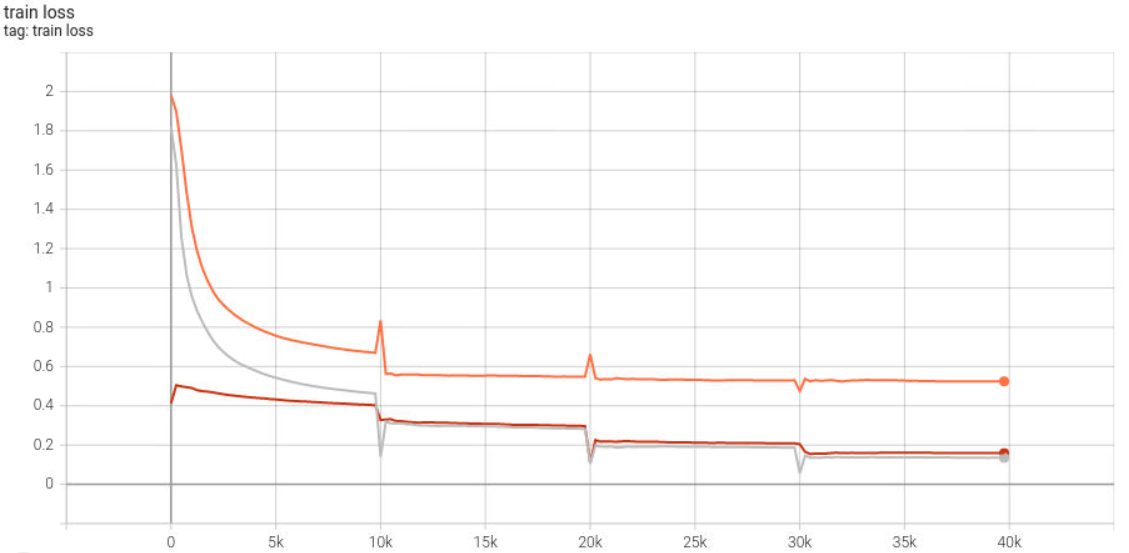
\includegraphics[width=0.5\textwidth]{pretrain.png} %插入图片,[]中设置图片大小,{}中是图片文件名
\caption{Utility of pretraining} 
\label{pic1}
\end{figure}

To see how it works, RNN is taken as an example. Both models in figure \ref{pic1} run under standard settings for thirty epochs. It is clear that RNN initialized randomly becomes overfitting after training for 5 epochs at the \emph{ppl} of 140, while, the blue curve, standing for the pretrained one decreases steadily and finally reaches the \emph{ppl} of 113. In contrast, the one initialized by the GoogleNews word vectors has only reached 151. It is no denying that pretraining help models make progress, but the task of pretraining has to be as relevant to the downstream task as possible.


\section{Conclusion}
During the second stage of the course, I build up various neural network models and conducted experiments to figure out relations between certain hyperparameters and model performance.
In addition, I compare models by their performance and try some popular tricks, such as pretraining, to make them work better.

Finally, I would like to give thanks to our tutors and seniors.
I have learned a lot and had a pretty good time in the last week!


\bibliographystyle{acl_natbib}
\bibliography{mycite}

\appendix

\section{Generate sentence}

Using the RNN initialized by pretrained word vectors, some words are provided for the model togenerate sentences by itself. The following are some examples.

\paragraph{sentence input:}
"in the past five years"
\paragraph{sentence output:}
"in the past five years is three pierre wachter group board appear once will factory" 

\paragraph{sentence input:}
"triggering a scramble among global"
\paragraph{sentence output:}
"triggering a scramble among global shame once will factory once editor is three is board" 

\paragraph{sentence input:}
"speculators are calling for a"
\paragraph{sentence output:}
"speculators are calling for a satisfaction is stopped which questionable is board once will factory"


\section{Records of experiments}

\begin{figure}[H] %H为当前位置,!htb为忽略美学标准,htbp为浮动图形
\centering 
\includegraphics[width=0.5\textwidth]{records.png} %插入图片,[]中设置图片大小,{}中是图片文件名
\caption{Records of experiments} 
\label{pic2}
\end{figure}


\end{document}
